% main_digest.tex — 5-page AEI digest of the IDD system paper.
% Standalone deliverable; the full 45-page manuscript (main.tex) is unaffected.
% article+twocolumn used instead of elsarticle (frontmatter+twocolumn double-typesets body text).
\documentclass[10pt]{article}

\usepackage[margin=2.2cm]{geometry}
\usepackage{amsmath,amssymb}
\usepackage{graphicx}
\usepackage{booktabs}
\usepackage{xcolor}
\usepackage[colorlinks=true,linkcolor=blue,citecolor=blue,urlcolor=blue]{hyperref}

\begin{document}


\begin{center}
{\LARGE\bfseries Trustworthy agentic diagnosis for industrial processes: a five-page digest}\par\vspace{10pt}
{\large ZhangHaoZheng}\par\vspace{2pt}
{\small Institute of Advanced Technology, University of Science and Technology of China, Hefei 230088, China}\par\vspace{14pt}
\end{center}
\begin{center}
\begin{minipage}{0.9\textwidth}
\small
\noindent\textbf{Abstract.} LLM-based root-cause analysis fails engineering practice for two reasons: conclusions cannot be audited, and benchmarks score sample-level classification where engineers need scenario-level, mechanism-grounded diagnoses. The Industrial Deep Diagnostic (IDD) pipeline answers with nine-stage agentic orchestration---ontology, deterministic statistics, competing-hypothesis reasoning, physical verification, quality gates with bounded repair---in which every conclusion decomposes into hypothesis, graded evidence (levels L1--L7), elimination, and a confidence bounded by cap-enforced ceilings. A machine-checked benchmark on 12 scenarios from SKAB, the Tennessee Eastman Process, and IndPenSim (nine documented faults, three normal controls) gives Top-1 resolution of 4/9 faults (44.4\%, Wilson 95\% CI $[18.9\%,73.3\%]$) with the true mechanism named in all nine surviving sets (top-$k$ 9/9), zero false alarms, and five capped \mbox{\textsc{competing\_set}} verdicts that name the measurement that would resolve them. A seeded random-draw re-execution reproduced the verdict state, actuator, and mechanism class within two confidence points; the deterministic baseline suite reproduces byte-for-byte. A model-controlled ablation bounds the accuracy claim: a bare call to the same model family resolves 9/9, so the pipeline's margin is auditable process, not accuracy. This digest condenses the full manuscript to five pages for editorial review.\par\vspace{4pt}
\noindent\textbf{Keywords:} fault root-cause analysis; large language models; multi-agent systems; evidence grading; reproducible benchmark.
\end{minipage}
\end{center}
\vspace{16pt}


\section{Background and position}
Root-cause analysis (RCA) of industrial anomalies asks a per-episode question---which correlated deviation is the cause, how confident are we, on what evidence---that classical fault detection and diagnosis scores only indirectly: PCA and deep detectors optimise sample-level labels~\cite{qin2012survey,tuli2022tranad}, with the TEP detection ceiling documented at IDV3/9/15 and weak $T^2$ response on IDV4~\cite{russell2000delay,chiang2001fault}. The closest LLM system, FaultExplainer~\cite{khan2024faultexplainer}, supplies candidate causes in its prompt and grades top-3 lists with alias acceptance; AgentRCA maintains a hypothesis table but reports no calibrated confidence~\cite{wei2026agentrca}. IDD's position, following the automation and trust literature~\cite{parasuraman2000model,lee2004trust} and Heuer's competing-hypotheses discipline~\cite{heuer1999psychology}, is that industrial diagnosis requires evidence policy, abstention~\cite{chow1970optimum,angelopoulos2023conformal}, and audit as machine-checked pipeline elements---not prompt conventions. Its named-discriminating-measurement exit is the passive counterpart of active fault diagnosis~\cite{scott2014input}: plant recordings arrive uncontrolled, so residual ambiguity is converted into an instrumentation request. The tripartite FDD lineage~\cite{venkatasubramanian2003review} and model-based diagnosis~\cite{isermann2005model} bound what is inherited rather than invented.

\section{The IDD system}
Fig.~\ref{fig:arch} shows the execution architecture as five planes. Fourteen interchangeable engines (Claude, OMP, Codex, ACP dialects, one-shot CLIs, a scripted mock) expose one uniform event contract with pre-flight probing and typed errors; the orchestrating main agent holds domain knowledge as 18 skill packages executed by 14 specialised agents and dispatches the diagnostic path to eight specialist sub-agents---context-builder, data-processor, diagnostician, judge, report-reviewer, reporter, html-visualizer, html-reviewer---that communicate only through workspace artifacts. A vision--language stage is nested inside the data-processor's Phase~5.5 and executed in its documented non-visual degradation here. Every stage transition appends a structured event to \texttt{.pipeline\_events.jsonl}; a log checker validates each agent's start/completion, declared outputs, and ordering, and a finalisation gate aggregates a 14-artifact inventory, JSON-schema validation, evidence closure, and the judge cross-audit into one PASS/FAIL verdict: no result exists without an execution proof.

The nine-stage pipeline (Fig.~\ref{fig:arch}, lower band) is strictly sequential with mechanical checkpoints CP-1\,\dots\,CP-9: ontology construction (CP-2/3, with deterministic fallback to a shipped mechanism map when the retrieval service is unreachable, as in every run reported here), statistics (CP-4), diagnosis (CP-5), the only mandatory parallel step---a ten-criterion judge and a physical pre-auditor (CP-6)---then report (CP-7), a final physical audit that must return ENDORSED (CP-8), manifest-first HTML build with independent review (CP-9), and script-side finalisation. Repair is bounded: best-of-3 per fault under a declared repair scope, a global cap of five, and an anti-oscillation confidence cap of 0.50; sub-threshold verdicts still ship with the cap recorded.

\begin{figure}[!t]
\centering
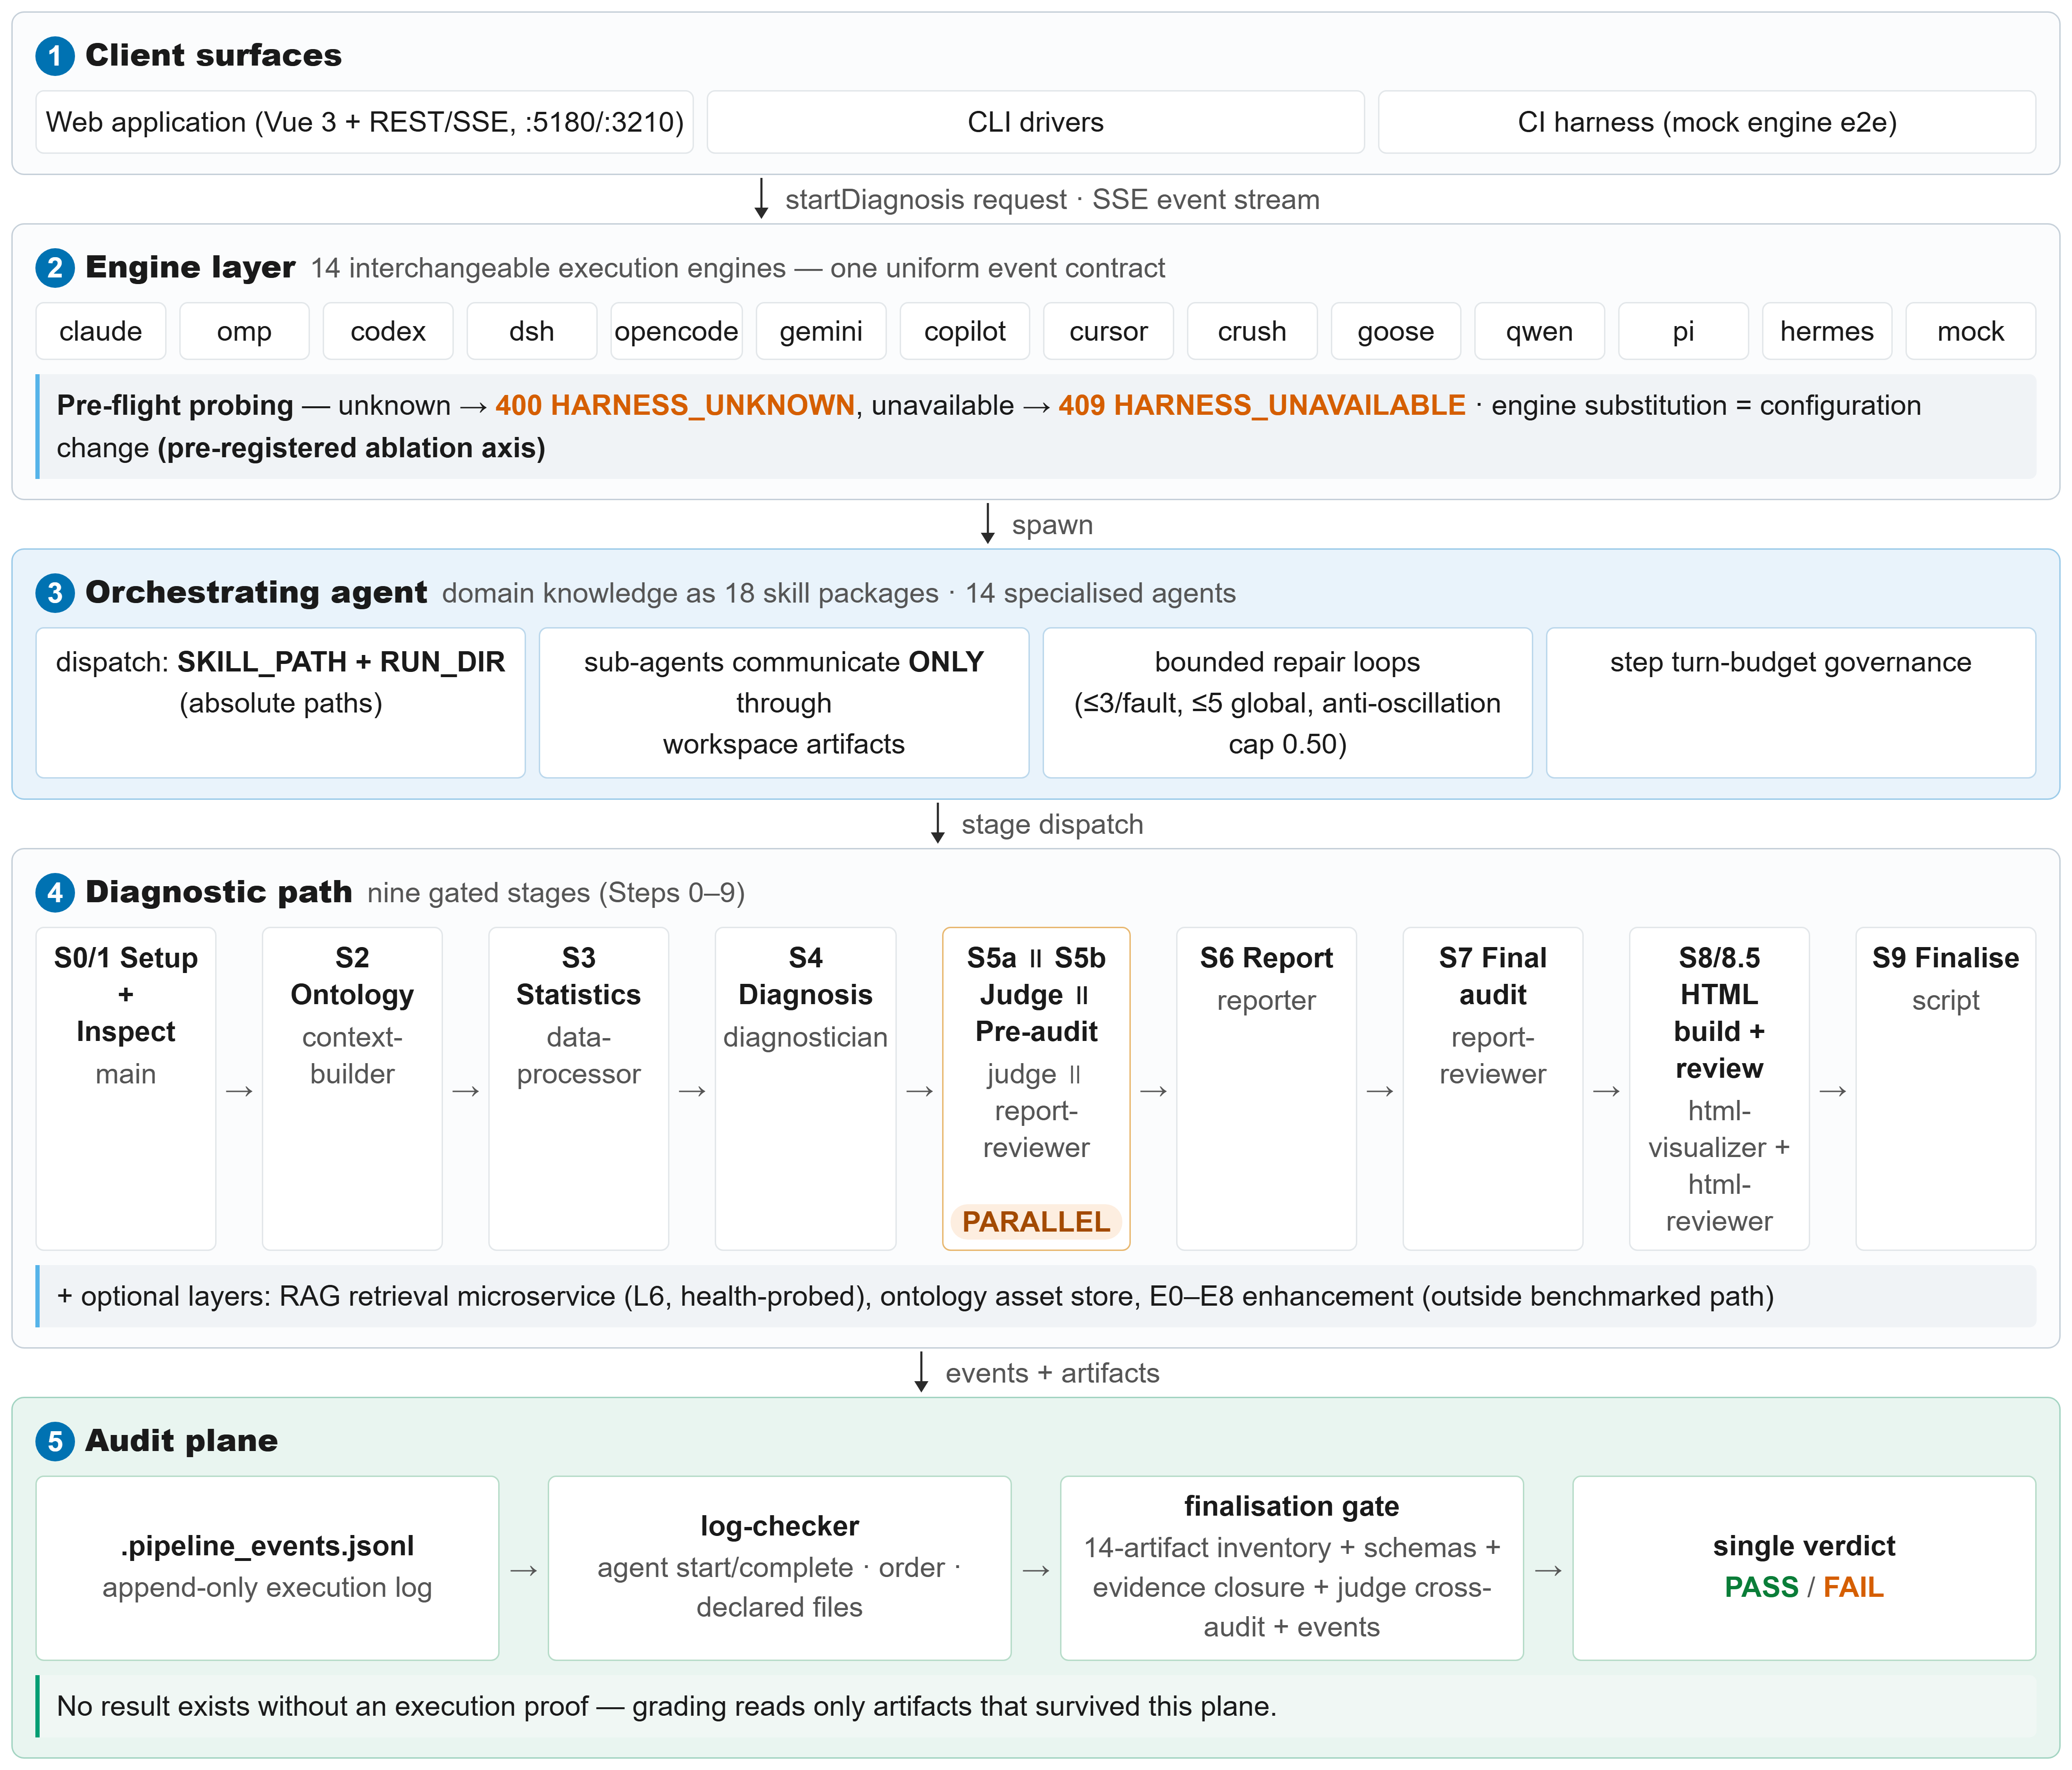
\includegraphics[width=0.82\textwidth]{../figures/fig_architecture.png}
\caption{Skill execution architecture: fourteen interchangeable engines behind one event contract; eight dispatched specialist sub-agents on the diagnostic path; every transition recorded on the audit plane whose log checker and finalisation gate produce the machine execution proof.}
\label{fig:arch}
\end{figure}

\section{Evidence-graded, three-state methodology}
Each scenario yields a verdict in \{\textsc{determined}, \textsc{competing\_set}, \textsc{needs\_data}\} with a mechanism, evidence chain, and confidence. Hypotheses carry mechanism classes and evidence levels L1--L7; a conclusion cannot exceed its weakest citation. Confidence is capped by the protocol: 0.70 for \textsc{competing\_set}, 0.65 for its indistinguishable subclass, 0.50 under anti-oscillation; the machine grading gate additionally enforces 0.90 for non-\textsc{cs} states at grading time. Four anti-spurious conditions gate every causal citation: lag-compensated temporal precedence, significance surviving detrending and multiple-testing correction, an ontology-annotated physical mechanism, and leave-one-out robustness under production-state filtering. Automatic physical verification recomputes balances and envelopes from the cleaned data, falling back to an explicit manual memo when no check applies. The verdict states are calibrated transfer, not evasion: a capped \textsc{competing\_set} localises the disturbance, eliminates families quantitatively, keeps the true mechanism ranked, and names the measurement that would collapse the set.

\section{Machine-checked benchmark and results}
The evaluation framework enforces five contracts: truth isolation with a two-directional leakage sentinel (keywords are grading-side only and author-designed, pinned at commit \texttt{221d061}), SHA-256 fingerprinting of all 153 inputs (re-verified at grading), stage-authored artifacts with provenance labels, gate-graded scoring (a scenario missing any of the fourteen artifacts is \emph{not executed}---a pipeline failure, not a result), and an artifact-consistency gate that recomputes every aggregate. The canonical runs executed as true per-stage sub-agent dispatches; the drawn re-execution ran fully sequential in $\approx$1.9\,h of agent time.

Table~\ref{tab:digest} and Fig.~\ref{fig:bench} summarise. IDD resolves 4/9 faults (TEP IDV1 A/C feed-ratio step 0.91, IDV7 header supply-capacity loss 0.78, IDV14 valve stiction 0.80, IndPenSim batch-93 cooling-actuator failure 0.82); determined-verdict precision is 4/4 and no control raises a false alarm. The five capped verdicts keep the true mechanism ranked in every case---two rank it first, three second of two---and name the discriminating measurement (suction-pressure spectra, steam-header and feed temperatures, the cooling-water inlet thermocouple). Within-family discrimination is statistics-driven: the three reactor-cooling perturbations separate into a step triad, a mean-frozen variance burst (actuator leading temperature by five samples, $r{=}{-}0.64$, the closed-loop lag-0 sign flip barred from causal citation), and a quantised-stepping stiction limit cycle. Consistency is tested by protocol: a seeded uniform draw (seed released) selected TEP IDV11 for full independent re-execution, which reproduced the verdict state, actuator XMV\_10, and mechanism class at $\Delta$confidence 0.02. The deterministic suite arms reproduce all 45 output files byte-for-byte with timestamps excluded; the artifact-consistency gate verifies 12/12 finalisation passes, 153/153 fingerprints, and recomputed aggregates. Two verdicts (0.91, 0.93) exceed the machine gate's flat 0.90 non-CS ceiling by 0.01/0.03---the measured gap between the agent-side and machine-side cap sets, recorded as rubric deductions.

\begin{table}[!t]
\caption{Digest of benchmark outcomes ($n{=}9$ faults, 3 controls; Wilson 95\% CI at $z{=}1.96$).}
\label{tab:digest}
\small
\begin{tabular}{@{}lcc@{}}
\toprule
Metric & Value & 95\% CI \\
\midrule
Resolved Top-1 (\textsc{det} and correct) & 4/9 & [18.9, 73.3] \\
True mechanism in surviving set (top-$k$) & 9/9 & [70.1, 100.0] \\
Determined-verdict precision & 4/4 & --- \\
Capped \textsc{cs} verdicts (truth ranked in all) & 5/9 & --- \\
Control pass / false alarms & 3/3 & [43.8, 100.0] \\
Verdict-type compliance & 8/9 & [56.5, 98.0] \\
Compliance rubric / judge gate (means) & 94.6 / 94.7 & --- \\
Finalisation gate & 12/12 PASS & --- \\
\bottomrule
\end{tabular}
\end{table}

\begin{figure}[!t]
\centering
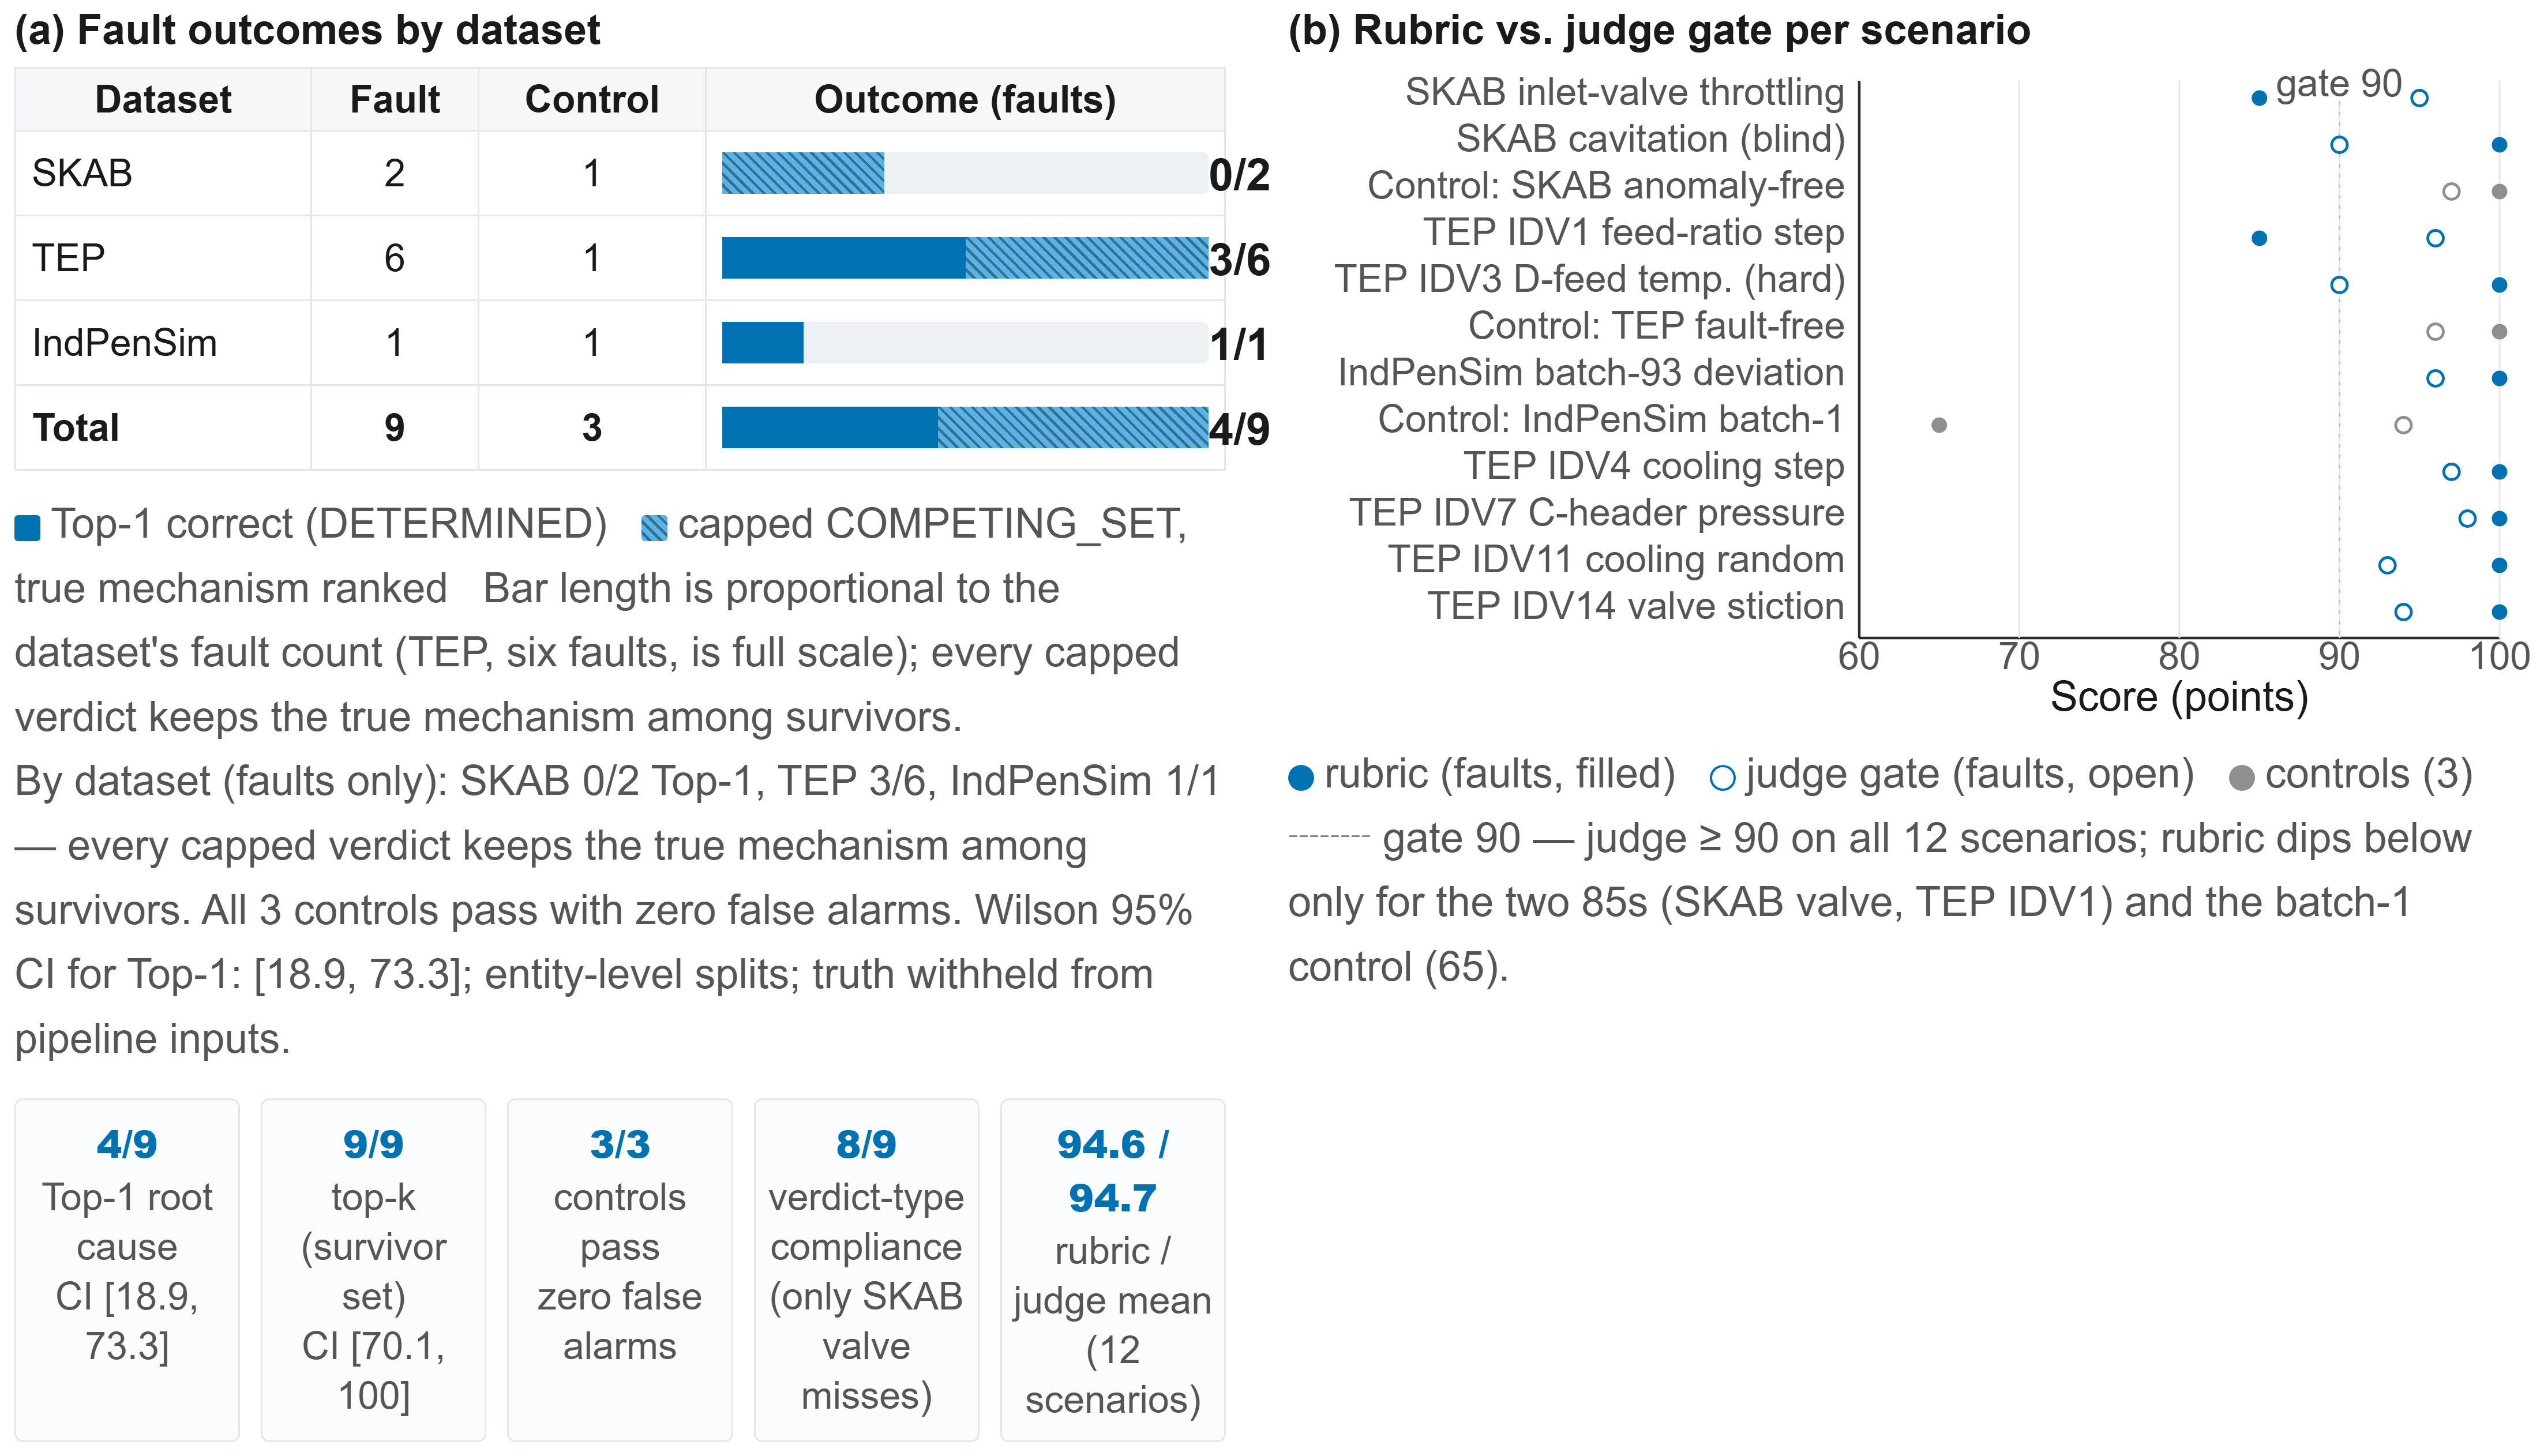
\includegraphics[width=0.93\textwidth]{../figures/fig_benchmark.png}
\caption{Benchmark outcomes. (a) Fault outcomes by dataset---Top-1-correct \textsc{determined} verdicts (dark blue) and capped \textsc{competing\_set} verdicts with the true mechanism ranked (hatched sky); all three controls pass. (b) Per-scenario deterministic rubric (filled) against the in-pipeline judge gate (open); dotted line: the judge's 90-point gate.}
\label{fig:bench}
\end{figure}

\section{Bounded claims and conclusion}
Three bounds frame the contribution. First, accuracy: the ablation shows a bare call to the same model family over the same blind digest resolves 9/9 against the pipeline's 4/9, so the pipeline's margin is the audit plane, cap-enforced uncertainty, execution proofs, and artifact provenance---not accuracy. Second, evidence: each headline is one recorded execution per scenario except IDV11's drawn re-execution; the remaining eleven scenarios carry explicit re-run contracts, and the rubric and keywords are author-designed instruments with expert anchoring outstanding. Third, cost: $\approx$1.9\,h of agent time per sequential diagnosis, amortised by the ontology-asset layer and meaningful against expert hours, not inference latency. What the five capped verdicts demonstrate is the transferable finding---diagnoses that route work: localise, eliminate, rank the truth, and name the channel to instrument next. The full manuscript (45 pages) carries the complete architecture, per-scenario evidence chains, consistency audit, and released artifact index; the evaluation repository accompanies the submission.

\bibliographystyle{elsarticle-num}
\bibliography{../refs}

\end{document}
